% !TeX root = thesis.tex

\chapter{Experiments}\label{ch:experiments}
In this chapter, we will discuss the experiments we conducted to evaluate the performance of our uncertainty-aware object detection model. 
We will describe the experiments done, present the obtained results, and analyze the performance of the model with a focus on its ability to capture and communicate uncertainty effectively.
Finally, we will analyze the results and discuss their implications for the use of uncertainty-aware models in robotic applications.

\section{Evaluation metrics}\label{ch:experiments_section:evaluation-metrics}
To measure how good the model is performing, we need to have a way to see if the model is accurate (the mean prediction is close to the target) and if the uncertainty is communicated well (the uncertainty of the predictions is high when the error is high, and low when the error is low).
This is a direct consequence of the chosen loss function, which is supposed to balance these two aspects.
There are a few ways we can evaluate the model's performance, each with their own focus and advantages.
The datapoints used for evaluation obviously need to be different from the datapoints used for training and validation to avoid data leakage.

\subsection{Loss Function}\label{ch:experiments_section:evaluation-metrics_subsection:loss-function}
The most obvious choise to evaluate a given model, is to use the loss function.
This is a great way to have a single number to compare the capability of the model while keeping the balance of the error and uncertainty.

It is the most important metric from a theoretical point of view, as it tells us exactly how well the model is at estimating its own weaknesses and strengths.
However, it is not the best metric to use for our use case, as it does not give us the ability to translate the loss into a value which has a clear meaning in our context.

\subsection{Uncertainty intervals}\label{ch:experiments_section:evaluation-metrics_subsection:uncertainty-intervals}
In the end, the models need to be used as a part of a robotic system without causing any harm to the environment.
We thus need a way to evaluate the model's performance in a way that can easily be translated into the real world.
Seeing that the model is outputting a mean and a variance, the step to statistical measures of error and uncertainty is quite small.

We want to be able to say something about the certainty of the error of the mean prediction.
For example, we want to be able to say that we are 95\% certain that the error that the mean prediction falls in a certain interval.
This means that the model can, with 95\% certainty, predict an interval of $[\bm{\mu}_\theta - \bm{\epsilon}, \bm{\mu}_\theta + \bm{\epsilon}]$ which contains the target value.
Note that the model is outputting a mean and a variance, both for the $x$ and $y$ coordinates of the target position, so $\bm{\mu_\theta}$ is a 2D vector.

The $\epsilon$, is a product of the $\sigma_\theta$ and the Z-score. 
The Z-score maps the desired confidence (for example, 95\%) level to a standard normal distribution where $\mu=0$ and $\sigma=1$.
\cref{eq:epsilon_calculation} shows how to calculate $\epsilon$ for a given confidence level $\alpha$ and a variance $\sigma^2_\theta$.

\begin{subequations}\label{eq:epsilon_calculation}
    \begin{align}
        \epsilon(\alpha, \sigma^2_\theta) &= z_\alpha \cdot \sigma_\theta \\
        \epsilon(\alpha, \sigma^2_\theta) &= z_\alpha \cdot \sqrt{\sigma^2_\theta}
    \end{align}
\end{subequations}
Note that the variables $\epsilon$, $\sigma_\theta$, and $\sigma^2_\theta$ are scalars, this thus holds in one dimension.
To go to two dimensions, we need to change one thing, the $z_\alpha$.
In one dimension, the $z_\alpha$ is a single value, but in two dimensions, we need to use a value from the chi-squared distribution with 2 degrees of freedom.
\cref{eq:epsilon_calculation_2d} shows how to calculate $\bm{\epsilon}$ for a given confidence level $\alpha$ and a variance $\bm{\sigma^2_\theta}$.

\begin{subequations}\label{eq:epsilon_calculation_2d}
    \begin{align}
        \bm{\epsilon}(\alpha, \bm{\sigma}^2_\theta) &= \sqrt{\bm{\chi}^2_\alpha} \cdot \bm{\sigma}_\theta \\
        \bm{\epsilon}(\alpha, \bm{\sigma}^2_\theta) &= \sqrt{\bm{\chi}^2_\alpha} \cdot \sqrt{\bm{\sigma}^2_\theta}
    \end{align}
\end{subequations}

Let's take a concrete example to make this more clear.
The model outputs a mean prediction of $\bm{\mu}_\theta=[50, 55]mm$ and a variance of $\bm{\sigma}^2_\theta=[4, 9]mm^2$.
We want to make an interval prediction with a confidence level of 95\%.
The $\chi^2$ value for 95\% confidence level and 2 degrees of freedom is 5.991.
Using \cref{eq:epsilon_calculation_2d}, we can calculate $\bm{\epsilon}$, which comes out to be $\bm{\epsilon}=[4.90, 7.34]mm$.
This then gives us the following interval prediction: 

$x \in [50 - 4.90, 50 + 4.90]mm$ and $y \in [55 - 7.34, 55 + 7.34]mm$.

These intervals, give a great way to evaluate the model's performance in a way that can be easily translated into the real world.

\subsection{Classifying predictions based on error and uncertainty}
Using the interval predictions from \cref{ch:experiments_section:evaluation-metrics_subsection:uncertainty-intervals} along with the target value, opens up the possibility to classify the predictions into different categories based on their error and uncertainty.
The following situations can occur:

\begin{itemize}
    \item The model is confident it will succeed in grasping the object, and it does. This is a \gls{tp}. This is the ideal situation, as the model is accurate and confident in its predictions.
    \item The model is not confident it will succeed in grasping the object, but it does. This is a \gls{fp}. This is a missed opportunity, as the model is timid
    \item The model is confident it will succeed in grasping the object, but it does not. This is a \gls{fn}. This leads to dangerous situations, as the model is overconfident.
    \item The model is not confident it will succeed in grasping the object, and it does not. This is a \gls{tn}. This is a safe situation, as the model is cautious when it should be.
\end{itemize}

To actually do this classification, we need to define the $max\_error$ the model can make while still grabbing the object successfully.
This is a value that can be defined based on the specific use case, which in our case is the radiance of the object to be grasped, which is 15mm.
This value is then translated, using \cref{eq:max_variance}, to a $maximum\_variance$ using the $\chi^2$ value for the desired confidence level and the number of dimensions, which is 95\% and 2 respectively in our case.

\begin{equation}\label{eq:max_variance}
    maximum\_variance = \frac{max\_error^2}{\chi^2_\alpha}
\end{equation}

This gives us all the necessary information to calculate whether a prediction's confidence is not misplaced (\cref{eq:confidence}), as well as whether the prediction is actually accurate enough (\cref{eq:success}).

\begin{subequations}
    \begin{align}
        max(\bm{\sigma}_\theta^2) &<= maximum\_variance \label{eq:confidence} \\
        \sqrt{\sum_{k=1}^{d}(\bm{\mu}_k - \bm{y}_k)^2} &<= max\_error \label{eq:success}
    \end{align}
\end{subequations}

If both of these conditions are satisfied, we have a \gls{tp}.
If the first condition is satisfied, but the second condition is not, we have a \gls{fp}.
If the first condition is not satisfied, but the second condition is, we have a \gls{fn}.
If both conditions are not satisfied, we have a \gls{tn}.

\subsection{Error-uncertainty graph}
The statistical scores are well to cevaluate and compare single instances given to the models.
The loss gives a general idea of how well the model is performing.
But both of these metrics fail to give a greater overview of how the model is performing over a greater set of samples.
The classification of predictions aids with this, but fails to communicate its hyperparameters and the severity of the errors and uncertainties.
A graph, like shown in \cref{fig:error-uncertainty-graph_example}, gives a better overview of the models performence over a greater set of samples and the hyperparameters.

\begin{figure}
    \centering
    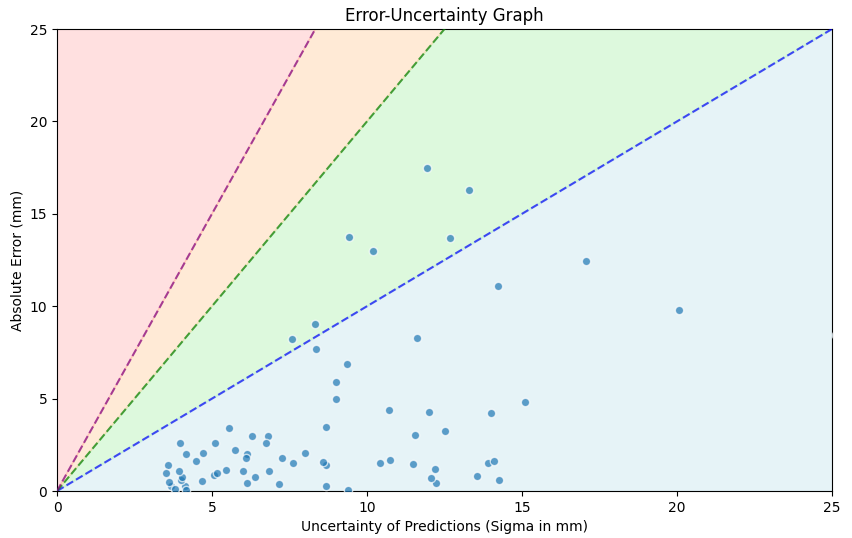
\includegraphics[width=1\textwidth]{static/error_variance_graph_example.png}
    \caption{An example of an error-uncertainty graph.}
    \label{fig:error-uncertainty-graph_example}
\end{figure}

The y-axis of the graph shows the uncertainty of a given prediction, this is the $\sqrt{\sigma_{\theta, i}^2}$ of the model's output.
The x-axis shows the error made by the model, this is calculated as $y_i - \mu_{\theta, i}$.
The graph is devided into 4 zones, each corresponding to a certainty level ($\alpha$) of the model's predictions:

\begin{itemize}
    \item Blue zone ($\alpha=0.68$): It is te be expected that 68\% of the predictions fall in this zone, as this is the center of the normal distribution. This is the "Cautious" zone, as the model is underconfident in its predictions.
    \item Green zone ($\alpha=0.95$): It is to be expected that 27\% of the predictions fall in this zone, as this is the area between the 68\% and 95\% confidence levels of the normal distribution. This is the "Sweet Spot" zone, as the model is well calibrated in this zone.
    \item Orange and red zone ($\lim_{\alpha \to 1}$): It is to be expected that 5\% of the predictions fall in this zone, as this is the area above the 95\% confidence level of the normal distribution. This is the "Danger" zone, as the model is blindly confident in its predictions while being way off.
\end{itemize}

\section{Experiment 1: Evaluating on a test set}\label{ch:experiments_section:evaluating-on-a-test-set}
The first test we conducted was to evaluate the model's on a test set.
This test set does not differ from the training and validation set in terms of the distribution of the data, but it does differ in terms of the specific samples used.
It would be expected that the models perform well on this and perform similarly to how they performed on the validation set.

\begin{table}[ht]
    \centering
    \begin{tabular}{c !{\vrule width 2pt} c|c|c|c|c}
        \textbf{Model index} & \textbf{Loss} & \textbf{TP} & \textbf{FP} & \textbf{FN} & \textbf{TN} \\
        \hline
        Deep Ensemble () & loss & TP & FP & FN & TN \\
        ResNet Ensemble () & loss & TP & FP & FN & TN \\
        MC Dropout () & loss & TP & FP & FN & TN \\
    \end{tabular}
    \caption{
        Comparison of the different models on the test set.
        }
    \label{tab:models_comparison_test_set}
\end{table}

\begin{figure}[]
    \centering
    \begin{subfigure}{0.49\textwidth}
        \centering
        
\includegraphics[width=\textwidth]{static/error-uncertainty-graph_deep-ensemble_1.png}
        \caption{Error-uncertainty graph for Deep Ensemble 1.}
        \label{sub_fig:error-uncertainty-graph_example_1}
    \end{subfigure}
    \hfill
    \begin{subfigure}{0.49\textwidth}
        \centering
        
\includegraphics[width=\textwidth]{static/error-uncertainty-graph_deep-ensemble_2.png}
        \caption{Error-uncertainty graph for Deep Ensemble 2.}
        \label{sub_fig:error-uncertainty-graph_example_2}
    \end{subfigure}
    \caption{Error-uncertainty graphs for the Deep Ensemble models on the test set.}
    \label{fig:Error-uncertainty-graphs_test-set_deep-ensembles}
\end{figure}

\section{Experiment 2: Evaluating on out-of-distribution data}\label{ch:experiments_section:evaluating-on-out-of-distribution-data}
\subsection{Multiple objects in the scene}
\subsection{Difficult lighting}
\subsection{Human intervention}